\documentclass[a4paper,11pt]{exam}
%\printanswers % pour imprimer les réponses (corrigé)
\noprintanswers % Pour ne pas imprimer les réponses (énoncé)
\addpoints % Pour compter les points
% \noaddpoints % pour ne pas compter les points
%\qformat{\textbf{\thequestion ) } }
%\qformat{\textbf{\thequestion )} \textit{(\thepoints)} \\  } % Pour définir le style des questions (facultatif)
\usepackage{color} % définit une nouvelle couleur
\shadedsolutions % définit le style des réponses
% \framedsolutions % définit le style des réponses
\definecolor{SolutionColor}{rgb}{0.8,0.9,1} % bleu ciel
\renewcommand{\solutiontitle}{\noindent\textbf{Solution:}\par\noindent} % Définit le titre des solutions

\usepackage{multicol}
\usepackage{caption}
\usepackage{tikz}
\usepackage{tkz-tab}
\usepackage{array}
\usetikzlibrary{trees}
\usepackage[final]{pdfpages}


\makeatletter

\def\maketitle{{\centering%
	\par{\huge\textbf{\@title}}%
	\par{\@date}%
	\par}}

\makeatother

\lhead{NOM Pr\'enom :}
\rhead{\textbf{Les r\'eponses doivent \^etre justifi\'ees}}
\cfoot{\thepage / \pageref{LastPage}}


%\usepackage{../../pas-math}
%\usepackage{../../moncours}


%\usepackage{pas-cours}
%-------------------------------------------------------------------------------
%          -Packages nécessaires pour écrire en Français et en UTF8-
%-------------------------------------------------------------------------------
\usepackage[utf8]{inputenc}
\usepackage[frenchb]{babel}
\usepackage[T1]{fontenc}
\usepackage{lmodern}
\usepackage{textcomp}



%-------------------------------------------------------------------------------

%-------------------------------------------------------------------------------
%                          -Outils de mise en forme-
%-------------------------------------------------------------------------------
\usepackage{hyperref}
\hypersetup{pdfstartview=XYZ}
%\usepackage{enumerate}
\usepackage{graphicx}
\usepackage{multicol}
\usepackage{tabularx}
\usepackage{multirow}


\usepackage{anysize} %%pour pouvoir mettre les marges qu'on veut
%\marginsize{2.5cm}{2.5cm}{2.5cm}{2.5cm}

\usepackage{indentfirst} %%pour que les premier paragraphes soient aussi indentés
\usepackage{verbatim}
\usepackage{enumitem}
\usepackage[usenames,dvipsnames,svgnames,table]{xcolor}

\usepackage{variations}

%-------------------------------------------------------------------------------


%-------------------------------------------------------------------------------
%                  -Nécessaires pour écrire des mathématiques-
%-------------------------------------------------------------------------------
\usepackage{amsfonts}
\usepackage{amssymb}
\usepackage{amsmath}
\usepackage{amsthm}
\usepackage{tikz}
\usepackage{xlop}
%-------------------------------------------------------------------------------



%-------------------------------------------------------------------------------


%-------------------------------------------------------------------------------
%                    - Mise en forme avancée
%-------------------------------------------------------------------------------

\usepackage{ifthen}
\usepackage{ifmtarg}


\newcommand{\ifTrue}[2]{\ifthenelse{\equal{#1}{true}}{#2}{$\qquad \qquad$}}

%-------------------------------------------------------------------------------

%-------------------------------------------------------------------------------
%                     -Mise en forme d'exercices-
%-------------------------------------------------------------------------------
%\newtheoremstyle{exostyle}
%{\topsep}% espace avant
%{\topsep}% espace apres
%{}% Police utilisee par le style de thm
%{}% Indentation (vide = aucune, \parindent = indentation paragraphe)
%{\bfseries}% Police du titre de thm
%{.}% Signe de ponctuation apres le titre du thm
%{ }% Espace apres le titre du thm (\newline = linebreak)
%{\thmname{#1}\thmnumber{ #2}\thmnote{. \normalfont{\textit{#3}}}}% composants du titre du thm : \thmname = nom du thm, \thmnumber = numéro du thm, \thmnote = sous-titre du thm

%\theoremstyle{exostyle}
%\newtheorem{exercice}{Exercice}
%
%\newenvironment{questions}{
%\begin{enumerate}[\hspace{12pt}\bfseries\itshape a.]}{\end{enumerate}
%} %mettre un 1 à la place du a si on veut des numéros au lieu de lettres pour les questions 
%-------------------------------------------------------------------------------

%-------------------------------------------------------------------------------
%                    - Mise en forme de tableaux -
%-------------------------------------------------------------------------------

\renewcommand{\arraystretch}{1.7}

\setlength{\tabcolsep}{1.2cm}

%-------------------------------------------------------------------------------



%-------------------------------------------------------------------------------
%                    - Racourcis d'écriture -
%-------------------------------------------------------------------------------

% Angles orientés (couples de vecteurs)
\newcommand{\aopp}[2]{(\vec{#1}, \vec{#2})} %Les deuc vecteurs sont positifs
\newcommand{\aopn}[2]{(\vec{#1}, -\vec{#2})} %Le second vecteur est négatif
\newcommand{\aonp}[2]{(-\vec{#1}, \vec{#2})} %Le premier vecteur est négatif
\newcommand{\aonn}[2]{(-\vec{#1}, -\vec{#2})} %Les deux vecteurs sont négatifs

%Ensembles mathématiques
\newcommand{\naturels}{\mathbb{N}} %Nombres naturels
\newcommand{\relatifs}{\mathbb{Z}} %Nombres relatifs
\newcommand{\rationnels}{\mathbb{Q}} %Nombres rationnels
\newcommand{\reels}{\mathbb{R}} %Nombres réels
\newcommand{\complexes}{\mathbb{C}} %Nombres complexes


%Intégration des parenthèses aux cosinus
\newcommand{\cosP}[1]{\cos\left(#1\right)}
\newcommand{\sinP}[1]{\sin\left(#1\right)}


%Probas stats
\newcommand{\stat}{statistique}
\newcommand{\stats}{statistiques}
%-------------------------------------------------------------------------------

%-------------------------------------------------------------------------------
%                    - Mise en page -
%-------------------------------------------------------------------------------

\newcommand{\twoCol}[1]{\begin{multicols}{2}#1\end{multicols}}


\setenumerate[1]{font=\bfseries,label=\textit{\alph*})}
\setenumerate[2]{font=\bfseries,label=\arabic*)}


%-------------------------------------------------------------------------------
%                    - Elements cours -
%-------------------------------------------------------------------------------




\usepackage{tabu}

%\usepackage{fullpage}
\author{\ }
\date{16 Mai 2019}
\title{$T^{le}$ $ST_2S$ : DS num\'ero 5}


\begin{document}
%	\usepackage{fancyhdr}
%	
%	\pagestyle{fancy}
%	\fancyhf{}
	%\rhead{Share\LaTeX}

	\maketitle





\section{Un QCM (6 points)}

\textit{Cet exercice se présente sous la forme d'un questionnaire à choix multiple (QCM). Pour chaque question, trois réponses sont proposées. Une seule réponses est correcte. On demande de choisir celle que vous pensez être correcte.
}


On donne le tableau de variation d'une fonction $f$ définie et dérivable sur l'intervalle $[-12, 20]$ :

\begin{center}

	\begin{tikzpicture}[scale=0.8]
		\tkzTabInit{$x$/1.5,$f'(x)$/1.5,$f(x)$/4}{$-12$, $-5$, $7$, $20$}
		\tkzTabLine { ,- ,z , +, z, -}
		\tkzTabVar{+/$7$,-/$-4$,+/$-1$,-/$-6$}
	\end{tikzpicture}

\end{center}

\begin{questions}
	\question[1] On peut dire que :
	
		\begin{checkboxes}
			\choice $f$ est positive sur l'intervalle $[-12; -5]$.
			\choice $f$ est positive sur l'intervalle $[7; 20]$.
			\correctchoice $f$ est négative sur l'intervalle $[-5; 20]$.
		\end{checkboxes}
	
		
	\question[1] L'équation $f(x)=2$ possède 
	
	\begin{oneparcheckboxes}
		
		\correctchoice une seule solution ;
		\choice aucune solution ; 
		\choice on ne peut pas répondre.
	\end{oneparcheckboxes}	

	\question[1] On cherche à comparer $f'(0)$ et $f'(8)$ :

\begin{oneparcheckboxes}
	
	
	\choice $f'(0) < f'(8)$
	\correctchoice $f'(0) > f'(8)$
	\choice on ne peut pas répondre.
\end{oneparcheckboxes}

	\question[1] On cherche à comparer $f(0)$ et $f(8)$ :
	
	\begin{oneparcheckboxes}
		
		
		\choice $f(0) < f(8)$
		\choice $f(0) > f(8)$
		\correctchoice on ne peut pas répondre.
	\end{oneparcheckboxes}



	\question[1] Une équation de la tangente à la courbe représentative de la fonction $f$ au point d'abscisse 20 est :
	
	\begin{oneparcheckboxes}
		
		
		\choice $y = 20x - 6$
		\choice $y = -x - 6$
		\correctchoice $y = -x + 14$
	\end{oneparcheckboxes}

	\question[1] On désigne par $\mathcal{C}$ la courbe représentative de $f$ dans un repère orthogonal.
	
	\begin{oneparcheckboxes}
		
		\choice Il n'existe aucun point où la tangente à la courbe $\mathcal{C}$ est parallèle à l'axe des abscisses.
		\choice Il existe un seul point où la tangente à la courbe $\mathcal{C}$ est parallèle à l'axe des abscisses.
		\correctchoice Il existe deux points où la tangente à la courbe $\mathcal{C}$ est parallèle à l'axe des abscisses.
	\end{oneparcheckboxes}	
\end{questions}

\newpage 

\section{Une épidémie (7 points)}

Une épidémie affecte une île du Pacifique, depuis le mois d'avril 2013. Nous disposons des données du nombre de personnes infectées sur les mois d'avril à septembre 2013. Ces données sont récapitulées dans le tableau suivant :

\vspace*{0.5cm} 
\begin{center}
	\begin{tabular}{|@{\ }l@{\ }|@{\ }c@{\ }|@{\ }c@{\ }|@{\ }c@{\ }|@{\ }c@{\ }|@{\ }c@{\ }|@{\ }c@{\ }|}
		\hline
		Mois                                & Avril      & Mai        & Juin & Juillet    & Août & Septembre \\ \hline
		Rang du mois $x_i$                  & 0          & 1          & 2    & 3          & 4    & 5         \\ \hline
		Nombre de malades en milliers $y_i$ & \num{17.5} & \num{27.5} & 35   & \num{42.5} & 49   & 51        \\ \hline
	\end{tabular}
\end{center}

\begin{questions}
	\question[1] En observant le nuage de points correspondant au tableau, tracé ci-dessous, un ajustement affine est-il envisageable ?
	\begin{solution}
		Oui, un ajustement affine est envisageable car le nuage de point est allongé.
	\end{solution}
	
	\question[1\half] Calculer les coordonnées du point moyen $G$ du nuage de points et l'ajouter sur le nuage de points.
	\begin{solution}
		Calcul des coordonnées du point moyen G :
		
		\begin{eqnarray*}
			\bar{X} &=& \frac{0 + 1 + 2 + 3 + 4 + 5 }{6}\\
			\bar{X} &=& \frac{14}{6}\\
			\bar{X} &=& \num{2.5}
		\end{eqnarray*}
	
		\begin{eqnarray*}
			\bar{Y} &=& \frac{\num{17.5} + \num{27.5} + 35 + \num{42.5} + 49 + 51 }{6}\\
			\bar{Y} &=& \frac{\num{222.5}}{6}\\
			\bar{Y} &\approx& 37			
		\end{eqnarray*}
	
		Donc les coordonnées du point G sont $(\num{2.5}; 37)$.
	\end{solution}
	
	\question[2] On considère la droite $(d)$, d'équation $y = \num{6.8} x + 20$, réalise un bon ajustement du nuage de points. Tracer la droite $(d)$.
	
	\question En utilisant l'approximation affine précédente, déterminer par le calcul :
	\begin{parts}
		\part[1\half] le nombre de personnes atteintes en février 2014 ;
		
		\begin{solution}
			Le mois 0 est avril 2013, il y a 10 mois entre avril 2013 et février 2014. Je cherche le nombre de malades pour le mois de rang 10  :
			
			\begin{eqnarray*}
				y &=& \num{6.8} x + 20 \\
				y &=& \num{6.8} \times 10 - 20\\
				y &=& 68 + 20 \\
				y &=& 88
			\end{eqnarray*}
			
			En février 2014 il y aura \num{88000} personnes atteintes.
		\end{solution}
		\part[1\half] le mois à partir duquel la population atteinte dépassera \num{10000} personnes.
		\begin{solution}
			Je cherche le rang du mois où on dépassera les  \num{10000} malades :
			
			\begin{eqnarray*}
				y &=& \num{6.8} x + 20 \\
				100 &\leq& \num{6.8} \times x + 20\\
				100 - 20 &\leq& \num{6.8} \times x \\
				80 &\leq& \num{6.8} \times x \\
				\frac{80}{\num{6.8}} &\leq& x \\
				\num{11.7} &\leq& x
			\end{eqnarray*}
			
			Il faudra attendre plus de 11 mois pour dépasser les \num{100000} personnes atteintes, soit avril 2014.
		\end{solution}
	\end{parts}
	
\end{questions}

\begin{center}
	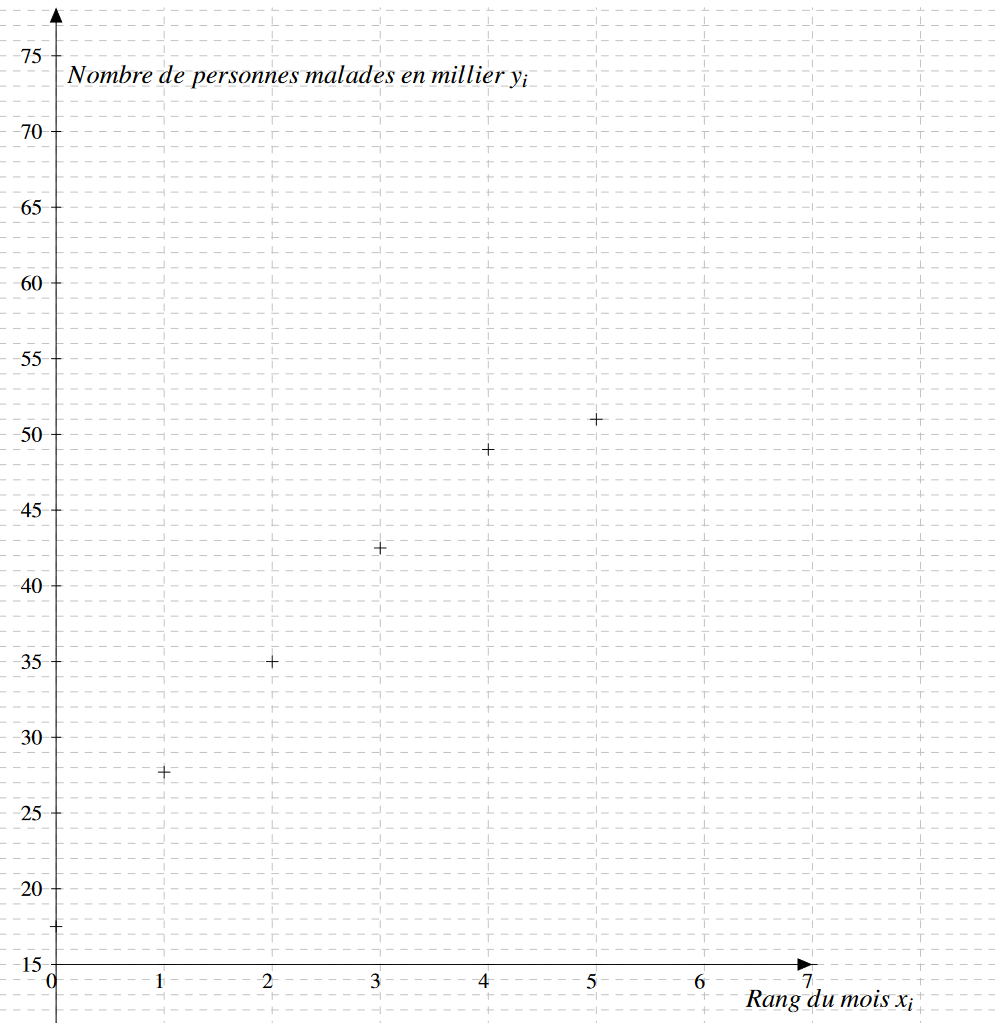
\includegraphics[scale=0.5]{nuage}
\end{center}

%\newpage 

\appendix

\section{Courbe représentative de la fonction $f$ de l'\ref{ex:deg3}}\label{app:fig}

%\begin{center}
	\begin{figure}[h]
		
		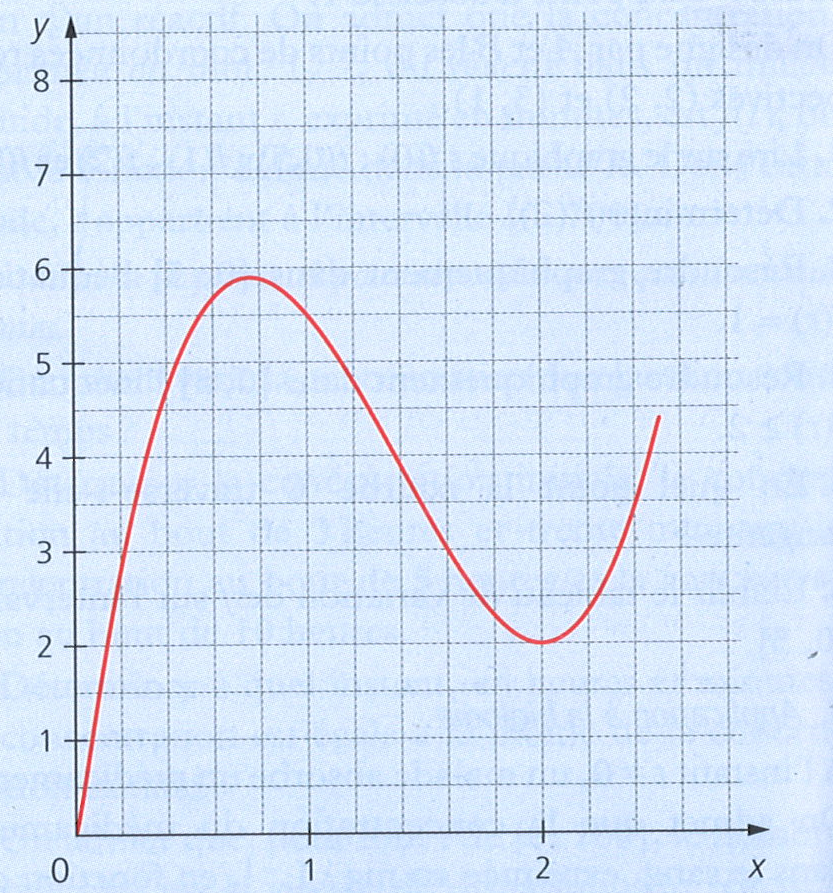
\includegraphics[scale=0.7]{img/courbe_31}
		
		\caption{Courbe $\mathcal{C}$}
		\label{fig:c}
	\end{figure}
%\end{center}

\label{LastPage}
	

\end{document}